\documentclass[12pt,oneside,openany,a4paper,%..... Layout
               afrikaans, english,%.............. Global language selection
               ]{memoir}

 \usepackage[masters-t,%.......................... Master thesis
             goldenblock,%........................ A5 type block (or a5block or wide)
            ]{usthesis}%.......................... US thesis style with memoir

%
% PLEASE read the USthesis documentation for the class options
% and how to set line and paragraph spacing
%

%==== Language setup ================================================
 \usepackage[latin1]{inputenc}%................... Recognizes �, �, etc
 \usepackage{babel}%.............................. Language setup

%==== Math setup ====================================================
 \usepackage{amsmath}%............................ Advanced math (before fonts)
 %\usepackage{amssymb}%............................ AMS Symbol fonts

%==== Font setup (default is Computer Modern) =======================
 \usepackage[T1]{fontenc}%........................ Type 1 fonts
 %\usepackage{fourier}
 \usepackage{textcomp}%........................... Additional text character
 \usepackage{bm}%................................. Bold math symbols (after fonts)

%==== Ref's, Bib's and Nomencl ======================================
 \usepackage{usnomencl}%.......................... List of symbols (in usthesis pack)
 \usepackage{usbib}%.............................. Bibliography    (in usthesis pack)
    \bibliographystyle{usmeg-a}
    \renewcommand\bibfont{\small}

    %% For usmeg-a, the bib is a list of references. If you
    %% are using usmeg-n comment out the following lines
    \addto{\captionsafrikaans}{\renewcommand{\bibname}{Lys van Verwysings}}
    \addto{\captionsenglish}{\renewcommand{\bibname}{List of References}}

%==== Graphics and Color ============================================
\usepackage{graphicx}%........................... Graphicx loaded in usthesis
\usepackage{color}%.............................. Color setup
\usepackage{eso-pic}%............................ Shipout commands for watermark
    \newcommand*{\WaterMark}[2][0.15\paperwidth]{%
        \AddToShipoutPicture*{\AtTextCenter{%
                \parbox[c]{0pt}{\makebox[0pt][c]{%
                    \includegraphics[width=#1]{#2}}}}}}

%==== Local Defs ====================================================
\makeatletter

%
% Please insert user defined commands here
% and NOT in the document itself!
%

\makeatother

%==== TITLE PAGE ====================================================
\title{\bfseries
       \AorE{%-- Afrikaans ------------------------------------------
             Diskrete Element Modellering van 'n Vibrerende Skeurploeg\\[1ex]
             \normalfont\small\itshape
             (``An Age Structured Model Of Substance Abuse'')
            }{%-- English -------------------------------------------
             An Age Structured Model Of Substance Abuse
            }}

\author{F.\ Chinake}{Filister Chinake}

\degree{\AorE{MIng (Meg)}{Masters  (Mathematics)}}
       {\AorE{Magister in Ingenieurswese (Meganiese)}
             {Master of Science}}

\address{\AorE{%-- Afrikaans ----------------------------------------
        Departement Meganiese en Megatroniese Ingenieurswese,\\
        Universiteit van Stellenbosch,\\
        Privaatsak X1, Matieland 7602, Suid Afrika.%
             }{%-- English ------------------------------------------
        Department of Mathematical Sciences,\\
        University of Stellenbosch,\\
        Private Bag X1, Matieland 7602, South Africa.
             }}

\faculty{\AorE{Fakulteit Ingenieurswese}%
              {Faculty of Mathematics}}

\supervisor{Prof.\ F.\ Nyabadza}
%\cosupervisor{Mnr.\ J.\ Smith}

\setdate{09}{2016}

%\SetSponsor{The financial assistance of the National Research Foundation (NRF)
%    towards this research is hereby acknowledged. Opinions expressed and
%    conclusions arrived at, are those of the author and are not necessarily to
%    be attributed to the NRF.}


%====================================================================
%     MAIN DOCUMENT
%====================================================================
\maxsecnumdepth{subsubsection}
\maxtocdepth{section}

\begin{document}

%==== Front matter ==================================================
 \frontmatter
 \WaterMark{UScrest-WM}
 \TitlePage

 \DeclarationDate{2016/09/10}
 \DeclarationPage

% \include{frontmatter/Chap-Front}

 \tableofcontents
 \clearpage

 \setcounter{lofdepth}{2}
 \listoffigures
 \clearpage

 \listoftables
 \clearpage

 %\chapter{Nomenclature}

\begin{Nomencl}
 \NomGroup{Constants}%-----------------------------------------------
   \item[$\mathrm{g} = $] $\mathrm{9.81\,m/s^2}$

 \NomGroup{Variables}%-----------------------------------------------
   \item[$\mathit{Re}_\mathrm{\,D}$]
                      \UnitLine{Reynolds number (diameter)}{~}
   \item[$x$]         \UnitLine{Coordinate                }{m}
   \item[$\ddot{x}$]  \UnitLine{Acceleration              }{m/s^2}\\
   \item[$\theta$]    \UnitLine{Rotation angle            }{rad}
   \item[$\tau$]      \UnitLine{Moment                    }{N{\cdot}m}

 \NomGroup{Vectors and Tensors}%-------------------------------------
   \item[$\overrightarrow{\bm{v}}$] Physical vector, see equation ...

 \NomGroup{Subscripts}%----------------------------------------------
   \item[$\mathrm{a}$] Adiabatic
   \item[$a$]          Coordinate
\end{Nomencl}



\endinput


%==== Main document =================================================
\mainmatter
   \setsecnumdepth{subsubsection}
%   \numberwithin{equation}{section}
%   \numberwithin{figure}{chapter}
%   \numberwithin{table}{chapter}

%\chapter{Introduction}



%%%%%%%%%%%%%%%%%%%%%%%%%%%%%%%%%%%%%%%%%%%%%%%%%%%%%%%%%%%%%%%%%%%%%%%
\section{Substance Abuse}
 
The substance abusing problem is complex and has widespread consequences. Various research findings have consistently pointed to the enormity of the problem worldwide. Research findings estimate that around $246$ million individuals were reported to have used an illicit drug in 2013, with $27$ million  reported to have progressed to become high risk drug users \cite{unodc2015}. High risk drug users is a new term referring to the group of people previously considered as the problem drug users. High risk drug use is defined by the American Monitoring Centre for Drugs and Drug Addiction (EMCDDA) as injecting drug use or long duration or regular use of opioids, cocaine and/or amphetamines \cite{EMCDA}.

The number one drug for which people seek treatment in Africa is cannabis. Substance abuse  in Africa is mainly fuelled  by the continent's role in illicit drug trafficking. Due to various factors the African continent is a transit route for drugs transported across the globe with South Africa considered the regional hub \cite{unodc2015}. Although the drugs into Africa are destined for Europe and North America the transit countries have a habit of becoming user countries \cite{segell1998stability}. As a result African countries are vulnerable to drug abuse along with crime related to drugs. Usually there is increase in organized crime thus further widening the  economic influence of traffickers threatening the security,health and development of the continent.
 
 Alcohol is reported as the most abused substance in South Africa \cite{parry1998substance}. The Western Cape province was reported to have the second highest prevalence of harmful drinking amongst expecting mothers \cite{harker2008substance} . High numbers of Foetal Alcohol Spectrum Disorders (FASD) signify the extend of alcohol abuse among women in the province. The rate of babies born with (FASD) in the province is reported to be among the highest in the country.Substance abuse is defined as the hazardous or harmful use of alcohol and  illicit drugs. Usually  people do not regard alcohol abuse as a real problem for which they should seek treatment. The Ministry of Social Development is mainly responsible for programmes that seek to address substance abuse issues in the Western Cape province. In order to accomplish the task it is imperative that at risk individuals are timeously identified in order for them to be given necessary help before they progress into dependence. 


Drug abuse in South Africa  is mainly driven by increased supply of drugs. Illicit drugs are easily available since the country is the largest transit zone in Africa. Poverty also drives the increase in street level dealing of illicit drugs. Other factors responsible for substance abuse amongst the youth population are family dysfunction and the phenomenon of absent parents. As the drug problem escalates the province is faced with even higher rates of gangsterism. Gangs have extended their turfs into schools where learners are being manipulated as mediums facilitating the sale of drugs in school premises. This has made schools very unsafe as they are characterised by gang violence and robbery.In the Western Cape province alone results from a survey of 133 schools revealed that  $61.6 \%$ of these schools had experienced gang related disturbances with $2$ out of every $5$ schools confirming the presence of drug merchants and peddlers within their schools \cite{socialdevelopwc}.

 In some communities drug dealing is so intricately interwoven into the community micro economics. This usually breeds powerful gang structures with leadership in place  exercising power through the patronage system and they become the source of employment especially in impoverished areas mostly characterised by high levels of unemployment. As these communities heavily depend on the income that comes from drug peddling this problem becomes so entrenched into the community and addressing the supply of drugs in such cases is very challenging and the resulting criminal network are extremely difficult to break\cite{modernisation}.
 
 Cape Town experiences high levels of substance abuse with most people reporting methamphetamine as their primary substance.  There has been an increase in demand of drug abusing treatment \cite{kalula2012theoretical} with methamphetamine accounting for $35 \%$ of patient admission . Other common drugs abused are alcohol and cannabis. The abuse of stimulants such as methamphetamine in Cape Town is also linked to other health related problems since they lead to a  rise in risky sexual behaviour \cite{harker2008substance} a as well as the escalation of social problems associated with abusing substances. 
 
 Various factors influence patterns in substance abuse. Age, social class, occupation, school status ,gender and geographical location are pivotal in establishing the extend of susceptibility of an individual to substance abuse. Peer pressure is what gets most young people involved in drugs amongst younger people. The culture of communal drinking promotes alcohol abuse among adults \cite{parry1998substance}.More factors to consider are chemical dependence on alcohol, poor social conditions and boredom as well as  a lack of social mechanisms that are pt in place to deal with people abusing alcohol and illicit drugs. Reasons why some people get involved in substance abusing activities range from habit, the need to alter mood states, a mechanism coping with stressful situations as well as a way of enjoyment.



Drug abuse is a chronic health condition which is difficult to control because in most places it is consider a criminal offence \cite{unodc2015}. Epidemiological indicators of substance abuse are usually estimated from incomplete data. This hinders efforts to monitor and control the spread of substance abuse  \cite{rossi2003role}. Information on substance abuse is obtained from general population and school surveys, estimates of problem drug use, data collected from treatment centres, information in relation to drug related deaths and also drug related infections such as HIV.

\section{Substances Abused In Cape Town}

\subsection{Methamphetamine}
$98\%$ of Tik addicts who seek help in South Africa are from the Western Cape \cite{mordenisation}. Methamphetamine is a powerful highly addictive stimulant which affects the central nervous system. The street name of the drug in Cape Town is called Tik. Worldwide methamphetamine goes by the name meth, chalk, ice and crystal. It is a white,  colorless, bitter-tasting crystalline powder that dissolves easily in water or alcohol. It is a drug that is medically used for patients who suffers from attention deficit hyperactivity disorder. It is also used as a short component of weight loss treatment . To the user the drug results in a pleasurable sense of well being or euphoria. Greater amounts of the drug gets into the brain and will cause longer lasting harmful effects to the central nervous system. This drug has a high potential for widespread abuse \cite{drugabuse1}.

\subsection{Alcohol}

Alcohol Use Disorder (AUD) is a medical diagnosis for problematic alcohol drinking that becomes severe \cite{nia}. Alcohol addiction is defined distinguished from alcohol abuse with addiction defined to be the psychological and physical dependence on alcohol while alcohol abusers are usually heavy drinkers, not necessarily addicted, who will perpetuate their drinking despite the consequences \cite{drug}.
Abusing alcohol has effects on the functioning of the body thus affecting the mood and behaviour of a person. Usually a person has difficulties thinking and making movement co-ordinations \cite{nia1}. Alcohol consumption is more common among farm workers around South Africa which is a result of the 'dop system' of the apartheid era. This refers to an arrangement where the employee is given alcohol as the benefit for employment \cite{london1999thedop}.  


\subsection{Cannabis}
Cannabis is commonly known as marijuana \cite{hall1998adverse}.Recreational users of cannabis perceive it as harmless. It is obtained from the plant Cannabis sativa and its subspecies. Cannabis contains $\Delta^9$ tetrahydrocannabinol (THC) responsible for marijuana intoxication resulting in its use for recreational purposes \cite{ashton1999adverse}.It can be smoked in hand rolled ,pipes, water pipes,smoked in blunts as well as mixing marijuana in food and ingesting it \cite{nidamarijuana}. The use of cannabis can result in mood altering effects such as euphoria. This ability to produce a high often results in wide spread and often chronic recreational use. Fatuous laughter and talkativeness often results if the substance is taken in a social gathering setting. In naive users the  most common side effects are anxiety, panic reactions, increased risk of accident as well as increased risk of psychotic symptoms (\cite{hall1998adverse},\cite{ashton1999adverse}). The long term use of cannabis increases the risk of respiratory cancer as well as acute and chronic bronchitis. Smoking in pregnancy is indicated for increased risk in birth defects such as ventricular septal defect and low birth weight \cite{csam}.

\section{Project Motivation And Objectives Of The Study}
\subsubsection{Motivation}
 Africa is no longer just the transit route for illicit drugs, but has also become the consumer of these drugs. This has made the problem more complex and leaves in its trail devastating effects \cite{au}. In some suburbs of Cape Town reports of violence and crime related to drug trafficking activities have increasingly become common. There is also a big challenge of providing support for the ever increasing number of drug users a direct result of drug trafficking activities in the city. One of the aims of the African Union as reported in their "Action plan on drug control (2013-2017)" is to increase monitoring of changing and emerging trends of drug use  as well as the implementation of evidence based responses \cite{au1}. To this end it is imperative that in order to gain understanding of the changing and emerging trends we need to consider important  characteristics that are influential in susceptibility to substance abuse. Age is one such factor that needs to be monitored and help detect the changing trends in relation to the substance abusing problem. To this end we seek to formulate an age related model of substance abuse.
\subsubsection{Objectives Of The Study} 
The main objective is to formulate a model of substance abuse incorporating age structure.
\\
Other objectives are:

\begin{itemize}
\item Determine if the model formulated is well posed.\\
\item Compute the basic reproduction number of the model formulated.\\
\item Choose a suitable numerical scheme for approximating the solution and determine its convergence.\\
\item Carry out numerical simulations of the age structured model of substance abuse.\\
\item Fit the model to the Cape Town Data for substance abusing people in rehabilitation.\\
\item To predict the trend of the age related substance abuse for the Cape Town population.\\
\item 
\end{itemize}

 
\section{Mathematical Preliminaries}
\subsection{The McKendrick-von Forster Partial Differential Equation}
The McKendrick equation gives a description of the time evolution of a population that is structured in age. It is one of the ways of modelling the evolution of an age structured population and it takes the form of the following partial differential equation:
\begin{equation}\label{McKendrickog}
\frac{\partial P(a,t)}{\partial t}+ \frac{\partial P(a,t)}{\partial a} = -\mu P(a,t)
\end{equation}

A standard way of solving equation (\ref{McKendrickog})is by using a method of characteristics. This method recognises the existence of curves 
\subsubsection{Method Of Characteristics}
There are curves in the a-t plane called characteristic curves. Along these curves the solution is constant and equal to its initial value.

In order to find the characteristic curves we introduce the following parametric curves
\[a=a(s) \quad \textsl{and}  \quad t=t(s)\]
 and we have the following
 \[K=P(a(s),t(s))\] taking 
 Thus we have 
 \begin{equation}
 \frac{dK}{ds}=\frac{dP(a(s),t(s))}{ds}=\underbrace{\frac{\partial P}{dt} \frac{dt}{ds} + \frac{\partial P}{ds}}_{\text{using the chain rule}}
 \end{equation}
 
 If we chose
 \begin{equation}\label{para1}
\frac{ da}{ds}=1 
 \end{equation}
 and 
 \begin{equation}\label{para2}
 \frac{dt}{ds}=1
 \end{equation}
 we have 
 \begin{equation}
 \frac{dK}{ds}=\frac{\partial P}{dt} +\frac{\partial P }{da}
 \end{equation}
 Eventually we get
 \begin{equation}\label{para3}
 \frac{dK}{ds}= -\mu(a(s)) K
 \end{equation}
 integrating equations(\ref{para1})and (\ref{para2}) we obtain the following characteristic curves
 \[t = t_0 +s \quad \text{and} \quad a=a_0 + s\]
 
 Integrating equation (\ref{para3}) we get 
 \begin{eqnarray}
  \int^{s}_{0} \frac{dK(\alpha)}{K(\alpha)}&=& -\int^{s}_{0} \mu (a(\alpha)) d \alpha \nonumber \\
  \text{ln} K(\alpha)]_{o}^{s}&=& -\int^{s}_{0}\mu (a_0 + \alpha)) d \alpha \nonumber \\
  \text{ln} [\frac{K(s)}{K(0)}] &=& -\int^{a_0 + s}_{a_0} \mu (\theta) d \theta \nonumber \\
  K(s) &=& K_0 e^{- \int^{a_0 + s}_{a_0} \mu (\theta) d \theta} \nonumber \\
  K(s) &=& K_0 \frac{e^{- \int^{a_0 + s}_{0} \mu (\theta) d \theta}}{e^{- \int^{a_0 }_{0} \mu (\theta) d \theta} }
\end{eqnarray}  
  
If we consider the initial condition $P(a,0)$
where $K(s)= P(a(s),t(s))$

Equating $P(a,0)= P(a(s),t(s))$  we get 
\[a(s)=a_0 + s= a\]
\[t(s)=t_0 +s =0\]

Taking \[t_0=0\Longrightarrow t=s \quad \text{and} \quad a_0=a-t\]
But we know that \[K(s)=P(a_0+s,s)\] and \[K(0)=P(a_0,0)=P(a-t,0)\]
Hence \begin{equation}
P(a,t)=P(a-t,0)e^{\int^{a}_{a-t} \mu (\theta) d \theta} \quad \text{for} \quad a >t
\end{equation}

If we consider the initial condition $P(0,t)$
where $K(s)= P(a(s),t(s))$

Equating $P(0,t)= P(a(s),t(s))$  we get 
\[a(s)=a_0 + s= 0\]
\[t(s)=t_0 +s =t\]

Taking \[a_0=0\Longrightarrow a=s \quad \text{and} \quad t_0=t-a\]
But we know that \[K(s)=P(s,t_0 + s)\] and \[K(0)=P(0,t-a)=P(0,t-a)\]
Hence \begin{equation}
P(a,t)=P(0,t-a)e^{\int^{a}_{0} \mu (\theta) d \theta} \quad \text{for} \quad t >a
\end{equation}
 \subsection{The Reproduction Number}
 The reproduction number denoted $R_0$ is defined as the average number of secondary cases generated by a primary case \cite{Chowell155}. This is an important measure in epidemiology that is used in assessing if an infection has the potential to spread in a population.
 
To obtain an expression for the basic reproduction number we make use of the Euler Lotka characteristic equation.
 
\subsubsection{The Euler Lotka Characteristic Equation}
 The Euler Lotka characteristic equation is given as 
 \begin{equation}\label{euler}
 \int_{\alpha}^{\beta} e^{-ra} m(a) l(a) da =1
 \end{equation}

where $l(a)$ is defined as the survival rate and $m(a)$ is defined as the maternity function depicting the birth rate per capita for mothers of age $a$.

Equation (\ref{euler}) has a unique solution $r_0$ which denotes the intrinsic rate of natural increase of a population. This is computed as the dominant real root of the Euler Lotka characteristic equation.

\subsection{Existence And Uniqueness Of Solutions}
One of the issues when dealing with a model that is given as a coupled set of partial differential equations is that it is not easy to derive an analytical solution to the system. As a result we appeal to a numerical solution that best approximates the solution.
Before resorting to a numerical implementation there are some issues that must first be verified. We need to determine if our system of equations is well posed. The main question to be ascertained is that do there exist a solution to our system? If that is satisfied we want the solution to be unique and to continuously depend upon the given initial data.
In order to establish the above conditions we formulate our system as an abstract Cauchy problem of the form

\begin{equation}\label{abstractcauchy1}
\frac{dx}{dt} = A x(t) + f(t,x) 
\end{equation}
The solution of the above equation can be established using the semi group approach as follows
\subsubsection{The Semi Group Approach}
If we consider the following differential equation
\begin{equation}\label{abstractcauchy2}
\frac{dx}{dt} = A x(t), \quad t \geq 0 , \quad x(0)=f \quad \text{on a Banach space X}
\end{equation}
 where $A$ is a given linear operator with domain $D(A)$ and $f \in X $.
 We obtain the generator $A$ of $T(.)$ which is given by setting 
 \[D(A)=\lbrace f\vert \text{lim}_{t\rightarrow 0^{+}} \frac{1}{t}(T(t)f-f) \quad \text{exists}\rbrace \] and is such that
 \[Af=\text{lim}_{t\rightarrow 0^{+}} \frac{1}{t}(T(t)f-f) \quad \text{for} \quad f \in D(A) \]
 
 
Since the generator defined above is a generator of a strongly continuous semi group $T(t)_{t\geq 0}$ we have that for every $f\in X$ the orbit map 
 \[x:t \longrightarrow x(t)=T(t)f\]
 is the unique mild solution of the abstract Cauchy equation (\ref{abstractcauchy2}) 
 
 
 
 
%\subsection{The Finite Difference Method}

\section{Outline Of The Thesis}
\chapter{Literature Review}
\section{Mathematical Models}

Mathematical models are a useful tool that explains the dynamics of a disease in population. Even the simplest of models does provide useful insights vital for understanding complex processes \cite{brauer2001mathematical}. A mathematical models allows for conceptual experiments that would be physically difficult or impossible to do \cite{aron2007mathematical}. We can extrapolate from available information to be able to predict how a disease outbreak will evolve. The ability to predict ensures that appropriate measures of curbing the spread of a disease through the whole population are put in place. Mathematical models are also a very useful tool for assessing the impact of these control measures \cite{keeling2009mathematical}.

\section{Models With Age Structure}
Structured population models distinguish individuals from one another according to characteristics such as age, size, location, status, and movement, to determine the birth, growth and death rates, interaction with each other and with environment, infectivity \cite{auger2008structured}



The age structured models capture the effects of demographic behaviour of individuals \cite{liu2015stability}. According to \cite{alexanderian2011age} age structured models are the most appropriate in the study of cholera since both vaccine efficacy as well as the risk of contracting cholera depends on the age of an individual. \cite{li2008continuous} emphasised on the fact that even the simplest models do cater for  some separate groupings in the population by dividing the population into different disease categories. They also highlighted that age may have some influence on reproduction, survival rates and behaviours. Here they noted that behavioural changes are very crucial as they are the major focus in the control and prevention of many infectious diseases. Let us also note that behavioural  changes are  an important aspect in the control and prevention of substance abuse.

Age structured models are used in studying various diseases and conditions. \cite{shim2006age} used to model the transmission of rotaries infection in the presence of maternal antibodies and vaccination. They made the  assumption that contacts between individuals are influenced by age-class activity levels as well age densities. Their population is divided into 6 age dependent classes where the age dependent mixing contacts structure is modelled via the mixing density $p(t,a,a')$ which gives the proportion of contacts between individuals of age $a$ and those aged $a'$ supposing that they have had some contact at time $t$. The basic reproduction and the control adjusted number are computed from the Lotka characteristic equation.


\cite{castillo2002age} discusses an age structured core group model and its impact on STD dynamics. An assumption of proportionate mixing is made and also assumes that the population has reached its stable distribution.In their work they apply the theorem that checks the two conditions, namely that $R_0 <1$ and $B$ is uniformly Lipshitz continuous on $\mathbb{R}^+$ to show that the disease free equilibrium is locally asymptotically stable. This is proved by applying the semi-group approach.

\section{Models Of Substance Abuse}

Epidemiological models are used to study the dynamics involved in the initiation and use of drugs because substance abuse is naturally contagious \cite{agestructureddrug}. In the case of infectious diseases there is need for an agent that is transmitted via physical contact while substance abuse is spread as an innovative socially acceptable practice to those susceptible to substance  abuse \cite{kalula2012}. Studying the evolution of substance abuse is more complex because we must not only consider the susceptible individual's immediate contacts as the only forces behind possible initiation. Another very influential force can be the overall perception of drugs in the susceptible person's society as sometimes portrayed in movies and news \cite{agestructureddrug}.

A common assumption in many models of substance abuse is that before a susceptible individual progress into the hard drug use state they are first recruited as light drug users(\cite{agestructureddrug},\cite{kalula2012},\cite{nyabadza2010}). The supporting assumption is also that light drug users provide a positive feedback that has more potential of initiating susceptible persons into substance abusing. On the other hand hard drug users are perceived negatively and alert people to the danger of substance abuse (\cite{agestructureddrug},\cite{kalula2012},\cite{nyabadza2010}).

Mathematical models have been formulated and explored in the province of Western Cape recently by ((\cite{kalula2012},\cite{nyabadza2010})). Other recent models of substances of substances have been formulated for other substances such as alcohol \cite{alcohol2007}.

Kalula and Nyabadza  considered a model for stimulants such as methamphetamine as the substance of abuse. This model divides the total population under consideration into core and non core groups . Six states are considered for the model where five states compartmentalise the population in the non core group.The model is shown to be well posed by establishing a feasible region that is positively invariant where the state variables remained non negative for positive initial  conditions. $R_0$ is defined to represent the average number of secondary cases that one drug user can generate in a population of potential drug users. $R_0$ is calculated using the next generation method. Numerical simulations to verify the theorem on stability of the drug free equilibrium are carried out using the Runge Kutta scheme in Matlab. A critical value of $R_0$ is established below which no drug persistent equilibria exists. It is not enough for $R_0 <1$ but for an effective drug abuse control the reproduction number must be brought below the critical reproduction number. The role of key parameters on the value of the reproduction number was investigated and it was established that reducing $R_0$ can be achieved by accelerating the rate of transference into the hard drug use compartment and the rate into the quitters compartment and into the rehabilitation compartment. The model proposes that in order to effectively fight the substance abusing problem it is imperative to limit the time spend in the light substance abusing compartment since these individuals are assumed to be more capable of recruiting more people than hard drug users. The data applied for the model was that of methamphetamine users in South Africa that sought treatment for the ten year period up to 2009 \cite{kalula2012}.

Nyabadza and Hove Musekwa formulated a model studying the dynamics of amphetamine use in the Western Cape Province. The aim of the model is to enable the prediction of the prevalence of drug use. Four compartments are included in the model. Data that was used for fitting was from the period of 1996 to 2008 which is the data for amphetamine abusers in treatment. An assumption of the model is that those who quit while in treatment move to the compartment of permanent quitters who can relapse after they have first recovered. Another very realistic assumption is that a quitter who relapses will most likely move straight into the hard drug user state because of the previous familiarity with abusing drugs. The incidence function includes an exponential function so as to cater for behaviour change in the model. Behaviour change is likely to result if a susceptible individual is exposed to the adverse effects of drugs such as death as they occur to a person already abusing substances. The model reproduction number is defined as the number of new initiates generated by one index case in a population that is entirely susceptible. It is a threshold number that determines the persistence of amphetamine abuse.
Reduction in reproduction number results in the reduction in the number of drug users. Practical ways as informed by the model is to reduce the contact rate between the susceptible and those on drugs, encourage increase in the behaviour change as well as reduce the time that those on drugs spend in the light drug use state where they have the greatest potential to recruit more susceptible people \cite{nyabada2010}.


The model considered by Fabio Sanchez et al  is a classic SIR epideomological framework where the population is divided into the compartments occasional and moderate drinkers (S) , problem drinkers (D) and temporarily recovered (R). Uptake into the susceptible class is considered as the number of new recruits that join the population as moderate and occasional drinkers. In the analysis of this model the drinking free equilibrium is defined as the state where a drinking culture does not exist. The reproduction number is thus  defined as the measure of resilience of the drinking free equilibrium to the invasion of problem drinkers. It gives the ratio of the average number of secondary cases generated by a typical drinker. Two forms of reproduction numbers are defined. A reproduction number $R_0 = \frac{\beta}{\mu}$ is defined in the absence of treatment and there is no class of those recovered from drug use yet. The other formulation of the reproduction number $R_{\phi}=\frac{\beta}{\mu + \phi}$ caters for the existence of recovered people after undergoing treatment. Clearly $R_0$ is greater than $R_{\phi}$ whenever $\phi$ is greater than 0. The implications of these  different reproduction numbers is that $R_0<1$ guarantees that the culture of drinking will not be established as long as the initial number of drinkers is low . On the other hand $R_0>1$ ensures that just the introduction of a single problem drinker will result in the eruption of a culture of drinking. $R_{\phi}<1$ does not guarantee that a culture of drinking will not be established because the $R$ class can produce more people who are  susceptible to alcohol abuse. The possibility of relapsing after recovering makes it imperative for treatment to be effective to avoid the blowing out of the alcohol abuse even with high rates of uptake into rehabilitation and quitting after treatment \cite{alcohol2007}.

Almeder et al formulated a model where the total population is divided into two groups mainly non- users and users. The model is simplified by disregarding the death and migration factors. They also assumed a constant birth cohort size. Movement is only one directional from the non user group to the user group.  User population does not just include the current users but includes everyone who has ever consumed or partaken of drugs.
The model describing the dynamics of non-users is given as a form of the McKendrick equation. This is given as 
\begin{eqnarray}
P_a + P_t = -\mu(a,t) P(a,t)
\end{eqnarray}
where in this case $\mu(a,t)$ represents the initiation rate whereas in our model this represents  the naturally mortality rate. 
This initiation rate $\mu(a,t)$ is assumed to be the product of three different factors namely a basic age specific initiation rate, the influence of the reputation of the drug as well as a prevention factor which includes the effects of age specific prevention programs \cite{agestructureddrug}.













\chapter{Model}

%In this chapter we formulate two models of substance abuse that are very similar and only differ with regard to the component that describes the force of infection. The first model assumes that the factor influencing initiation after contact between a susceptible and a substance abuser is innovation on the part of the susceptible. \citep{Bruno} describe the innovators as that type of individuals who make a decision to adopt a certain other people in the society or their interaction with peers.
%
%The other model assumes that the factor at play in the individuals that are recruited from the susceptible population to the drug users population is imitation. \citep{Bruno} also gives a description of these individuals as adopters who respond  to the pressure of their environment and thus it influences the timing of innovation not necessarily depending on the decision of their adoption.

In formulating the age structured model of substance abuse  we introduce the following parameters :

\begin{table}[h!]
\centering
\begin{tabular}{|c|l|}\hline
\text{Parameter} &\text{ Description}\\ \hline 
N(a,t) & \text{Expected population size  of age $a$ at time $t$}\\
\beta(a,t) & \text{The effective contact rate of age $a$ at time $t$}.\\
\mu (a) & \text{The per capita death rate as a function of age} \\
\sigma (a) & \text{The rate of movement into rehabilitation} \\
\gamma (a) & \text{The rate of relapsing while in rehab}\\
\rho(a) & \text{The recovery rate}\\
\omega (a) & \text{The relapse rate of the recovereds}\\
\alpha (a) & \text{The imitation coefficient} \\
\hline 

\end{tabular}
 \caption{The table gives the model parameters and their description.}
\end{table}







%N is a large positive integer, $\beta$ and $\mu$ are positive.
%\text{Parameter} &\text{ Description}\\ 
%N & \text{Expected population size  in case there are no infected individuals}\\
%
%
%\beta &\text{The contact rate between infectives and susceptibles}.\\
%\mu & \text{The death rate and the birth rate} \\
%\sigma & \text{The rate of movement into rehabilitation} \\
%\gamma & \text{The rate of relapsing while in rehab}\\
%\rho & \text{The recovery rate}\\
%\omega & \text{The relapse rate of the recovereds}\\
%\alpha & \text{The imitation coefficient} \\
%\end{array} \]


\section{Model Formulation}
Here we formulate a model that monitors four populations in relation to substance abuse. The first group consist of individuals  susceptible to substance abuse denoted by $S(a,t)$. These are individuals that are recruited into the population through birth. The second group is a group of drug users that are not in rehabilitation and that is denoted by $D(a,t)$. These individuals are initiated into drug use from the susceptible group. The  third compartment consists of individuals who are in rehabilitation having been in compartment $D(a,t)$ . The last compartment $Q(a,t)$ consists of individuals who have stopped using drugs and they are called  quitters. The total population is thus given by \[N=N(a,t)=S(a,t)+D(a,t)+R(a,t)+Q(a,t).\]
%Since the birth rate is equal to the death rate,  the population is assumed to be constant thus we have \[\frac{dN(t)}{dt}=0.\]
%This implies that \[\frac{dS(t)}{dt}+\frac{dD(t)}{dt}+\frac{dR(t)}{dt}+\frac{dQ(t)}{dt}=0.\]

The main assumption of this model is that the population is approximately constant within the modelling time. We also assume that that there is a homogeneous mixing among all individuals from different compartments. The class responsible for initiation is $D(a,t)$ which consists of drug users not in treatment. Drug users who are undergoing treatment in compartment $R(a,t)$ are assumed not to initiate new cases  since we assume that the rehabilitation is inpatient. We also assume that the susceptible class $S(a,t)$ consists of people who have never been involved in abusing substances before. Thus those who quit do not necessary move back to $S(a,t)$ but there is a possibility that they can still relapse and move straight back into $D(a,t)$. We now give the description of the dynamics of all compartments. The description is aided by  figure \ref{diagram}.

\begin{figure}[h!]
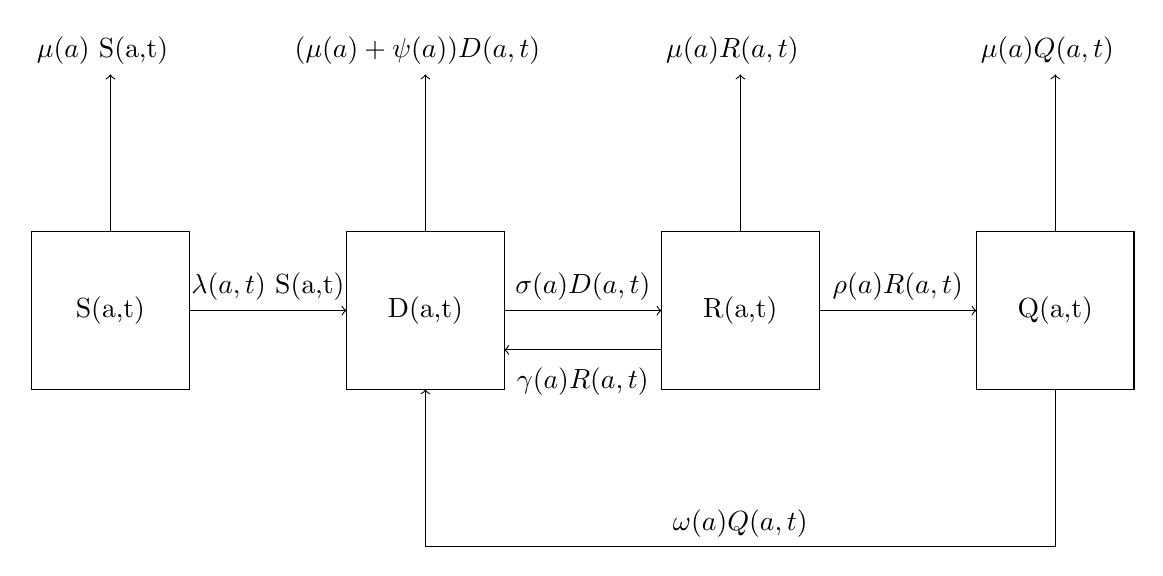
\begin{tikzpicture}
%\draw [->](-2,1) -- (0,1);
\draw  (0,0)rectangle(2,2) ;
\node (S) at (1,1) {S(a,t)};
\draw  (4,0)rectangle(6,2);
\node (D) at (5,1) {D(a,t)};
\draw  (8,0)rectangle(10,2);
\node (R) at (9,1) {R(a,t)};
\draw  (12,0)rectangle(14,2);
\node (Q) at (13,1) {Q(a,t)};
\draw [->] (2,1) -- (4,1);
%\node (1) at (-3,1) {$\mu$ N};
\draw [->] (6,1) -- (8,1);
\draw [->] (10,1) -- (12,1);
\draw [-] (13,0) -- (13,-2);
\draw [-] (13,-2) -- (5,-2);
\draw [->] (5,-2)--(5,0);
\draw[->](1,2) -- (1,4);
\node (2) at (0.9,4.3) {$\mu(a)$ S(a,t)};
\node (3) at (3,1.3) {$\lambda(a,t)$ S(a,t)};
\draw[->] (5,2) -- (5,4);
\draw[->] (9,2) -- (9,4);
\draw[->] (13,2) -- (13,4);
\draw[->] (8,.5) -- (6,.5);
\node (4) at (7,1.3) {$\sigma(a) D(a,t)$};
\node (10) at (7,.1) {$\gamma(a) R(a,t)$};
\node (5) at (11,1.3) {$\rho(a) R(a,t)$};
\node (6) at (4.9,4.3) {$(\mu(a)+\psi(a))D(a,t)$};
\node (7) at (8.9,4.3) {$\mu(a) R(a,t)$};
\node (8) at (12.9,4.3) {$\mu(a) Q(a,t)$};
\node (9) at (9,-1.7) { $\omega(a) Q(a,t)$};
\end{tikzpicture}
\caption{The diagrammatic representation of the substance abuse model with the compartments densities S(a,t),D(a,t),R(a,t),Q(a,t) and $\mu(a), \gamma(a), \sigma(a), \omega(a), \lambda(a), \rho(a)$ denoting the transition rates which are $\geq 0.$\label{diagram}}  
\end{figure}

\subsection{Susceptible Individuals, S(a,t)}
This is a group of individuals who are at risk of getting addicted to drugs. Individuals in this compartment have no history of substance abuse. Recruitment  into the susceptible compartment is due to births that are denoted by the boundary condition given below. Susceptible individuals initiated into substance abuse with an initiation function $\lambda(a,t)$ that is synonymous to the force of infection in disease models . The susceptible population is depleted through natural death plus disease induced death.
% Our general equation for this compartment is thus given as:
%\begin{eqnarray}\label{eq:sus}
%\frac{dS}{dt} & = &\mu N -\mu S - \lambda S 
%\end{eqnarray}

%%We are going to consider two forces of initiation. For the first one we assume that the force that drives the susceptibles into the drug using state is innovation on the the part of the susceptible individual due to interaction with individuals in $D$. The force of initiation is given as $\frac{\beta D}{N}$. 
The differential equation explaining the dynamics of the susceptible population is
 \begin{eqnarray}\label{inovation}
 \frac{\partial S(a,t)}{ \partial t}+ \frac{\partial S(a,t)}{\partial a} & = & -\mu(a) S(a,t) -\lambda(a,t)S(a,t). 
 \end{eqnarray}


%We also consider the case where the susceptible population is assumed to be recruited mainly through imitation.We introduce $\alpha$  which is an imitation coefficient. The parameter $\lambda$ becomes $\frac{\beta(1+\alpha D)D}{N}$. 
%This can be written as $\frac{\beta D}{N}+\frac{\beta \alpha D^2}{N}$. 
%It is clear that if $\alpha =0$ then the force of initiation is the same as in (\ref{inovation}).
% The corresponding differential equation that explains the dynamics of the susceptible population when there is a force of imitation is
%\begin{eqnarray}
%\frac{dS}{dt} & = &\mu N -\mu S - \frac{\beta(1+\alpha D)D}{N} S.
%\end{eqnarray}

%So the differential equation describing the dynamics of the susceptible population 
%%\begin{eqnarray}
%%\frac{dS}{dt} & = &\mu N -\mu S - \lambda S %\quad \text{where} \lambda \quad = \bigwedge 
% where 
%\[ \lambda = \left\{
%  \begin{array}{l l}
%    \frac{\beta D}{N} & \quad \text{if the force of infection is initiation only.}\\
%    \frac{\beta(1+\alpha D)D}{N} & \quad \text{if there is an extra imitation force.}
%  \end{array} \right.\]


\subsection{Drug Abusing Individuals, D(a,t)}

The individuals in this compartment are from the susceptible compartment as a result of contact. They are recruited at a rate $\lambda(a)$. Some of the people in this compartment are from the Rehabilitation compartment who relapse at rate $\gamma (a)$. Some of them come from the quitters compartment at a rate $\omega (a)$. These are the individuals who revert back to abusing drugs after recovering.
Individuals exit compartment $D(a,t)$ as a result of death at a rate equal to $\mu(a)+ \psi (a)$. Some are recruited into rehabilitation at a rate $\sigma(a)$.
The differential equation explaining the dynamics of this compartment are given as
\begin{eqnarray}
\frac{\partial D(a,t)}{\partial t} + \frac{\partial D(a,t)}{\partial a}& = &\lambda(a) S(a,t)+ \gamma(a) R(a,t) + \omega(a) Q(a,t)-(\mu(a)  +\sigma(a)+ \psi(a))D(a,t)
\end{eqnarray}

\subsection{Individuals in rehabilitation, R(a,t)}
Individuals in this compartment are taking corrective measures to stop abusing drugs. All of them are coming from $D(a,t)$. This compartment decreases due to death and progression to the quitters compartment. Some of them unfortunately revert back to abusing substance due to the process usually referred to as relapsing. The corresponding differential equation is
\begin{eqnarray}
\frac{\partial R(a,t)}{\partial t} + \frac{\partial R(a,t)}{\partial a} &= &\sigma(a) D(a,t)-(\mu(a) +\rho(a) +\gamma(a) )R(a,t).
\end{eqnarray} 
\subsection{Quitters, Q(a,t) }
Through rehabilitation there is a possibility of a complete recovery of individuals abusing substances. These individuals progress to compartment $Q(a,t)$ at a per capita rate $\rho(a)$. We allow these people not to quit permanently but have a chance to reuse drugs. When they relapse they progress to compartment $D(a,t)$ at a per capita rate $\omega(a)$. With a natural mortality rate $\mu(a)$, the dynamics of compartment $Q(a,t)$ is given by 
%The population of people in this compartment are recruited from the Rehabilitation compartment only. The assumption is that in order for any drug abusing individual to quit they first have to undergo treatment in the form of rehabilitation. However a recovered drug addict does not become immune to the disease hence some of them relapse back to the D compartment at a rate $\omega$.
\begin{eqnarray}
\frac{\partial Q(a,t)}{\partial  t}+\frac{\partial Q(a,t)}{\partial a} & = &\rho(a) R(a,t)-(\mu(a) +\omega(a)) Q(a,t). 
\end{eqnarray}
The  model diagram and assumptions leads to the following system of differential equations;
\begin{eqnarray}\label{model1}
\frac{\partial S(a,t)}{\partial t}+ \frac{\partial S(a,t)}{\partial a} & = & -\mu(a) S(a,t) -\lambda(a,t)S(a,t),\nonumber\\
\frac{\partial
D(a,t)}{\partial t} + \frac{\partial D(a,t)}{\partial a}& = &\lambda(a,t) S(a,t)+ \gamma(a) R(a,t) + \omega(a) Q(a,t)-(\mu(a)  +\sigma(a)+\psi (a)) D(a,t), \nonumber \\
\frac{\partial R(a,t)}{\partial t} + \frac{\partial R(a,t)}{\partial a} &= &\sigma(a) D(a,t)-(\mu(a) +\rho(a) +\gamma(a) )R(a,t), \nonumber \\
\frac{\partial Q(a,t)}{\partial t}+\frac{\partial Q(a,t)}{\partial a} & = &\rho(a) R(a,t)-(\mu(a) +\omega(a)) Q(a,t) . 
\end{eqnarray}

We assume that the number of births and deaths are balanced and also that the number of births is equal to the number of people aged zero such that we have 
\begin{equation}
N(0,t)= S(0,t)
\end{equation}
 
As a result we have the following boundary conditions:
\begin{equation}
S(0,t)= \theta(t) \quad \text{and} \quad D(0,t)=R(0,t)=Q(0,t)=0
\end{equation}

Adding the boundary conditions we get:
\begin{eqnarray}
N(0,t)&=& S(0,t)+D(0,t)+R(0,t)+Q(0,t)
       = \theta(t).
\end{eqnarray}
If we add up equations in (\ref{model1})
we get 
\begin{equation}
\frac{\partial N(a,t)}{\partial t}+ \frac{\partial N(a,t)}{\partial a}=-\mu N(a,t)-\psi(a) D (a,t)
\end{equation}

%Assuming $\psi$ to be very small such that $\psi \approx 0$ we get 
\begin{equation}\label{Mckendrick}
\frac{\partial N(a,t)}{\partial t}+ \frac{\partial N(a,t)}{\partial a} \leq-\mu N(a,t)
\end{equation}

We can see that equation (\ref{Mckendrick}) is a von McKendrick Form with a solution of the form

\[ N(a,t) \leq
  \begin{cases}
    \theta (t) e^{-\int\limits_{0}^{a} \mu(\epsilon) \mathrm{d}\epsilon}
       & \quad \text{if } a \leq t\\
    N(a-t,0) e^{-\int\limits_{a-t}^{a} \mu(\epsilon) \mathrm{d}\epsilon} 
       & \quad \text{if } a \geq t\\
  \end{cases}
\]
%\section{The Biologically Feasible Region}
%
%All the parameters and state variables of our model are non negative for all $t \geq 0$ we have the following feasible region :
%
%\begin{eqnarray*}
%Z_1 &=&\lbrace(S+D+R+Q) \in \mathbb{R}_{+}^{4}:S+D+R+Q \leq \theta (t) e^{-\int_{0}^{a} \mu (\epsilon) d \epsilon} \quad \text{if} \quad a \leq t \rbrace \\
%Z_2& = &\lbrace(S+D+R+Q) \in \mathbb{R}_{+}^{4}:S+D+R+Q \leq N(a-t,0) e^{-\int_{0}^{a} \mu (\epsilon) d \epsilon} \quad \text{if} \quad a \geq t \rbrace
%\end{eqnarray*}
%
%
%
%$Z_1$ and $Z_2$ are positively invariant $\forall t \geq t$.
%The deterministic version of the model with imitation   is given by the following system of differential equations;
%
%\begin{eqnarray}\label{imitation}
%\frac{dS}{dt} & = &\mu N -\mu S - \frac{\beta(1+\alpha D)D}{N} S, \nonumber \\
%\frac{dD}{dt} & = &\frac{\beta(1+\alpha D)D}{N} S+ \gamma R +\omega Q-(\mu +\sigma) D  ,\nonumber \\
%\frac{dR}{dt} &= &\sigma D-(\mu +\rho + \gamma) R , \nonumber \\
%\frac{dQ}{dt} & = &\rho R-(\mu +\omega )Q  .
%\end{eqnarray}

\section{Rescaling The Parameters}
%For the derivation of diffusion approximations of the stochastic version of the model it will be convenient to introduce
 We introduce the scaled state variables:
%$ \lambda=\frac{\beta D}{N}$ ,
 $s(a,t)=\frac{S(a,t)}{N(a,t)}$, $d(a,t)=\frac{D(a,t)}{N(a,t)}$, $r(a,t)=\frac{R(a,t)}{N(a,t)}$ and $q(a,t)=\frac{Q(a,t)}{N(a,t)}.$

Below is the rescaled version of equation (\ref{model1})
 \begin{eqnarray}\label{model2}
\frac{\partial s(a,t)}{\partial t}+ \frac{\partial s(a,t)}{\partial a} & = &  -\lambda(a,t)s(a,t),\nonumber \\
\frac{\partial
d(a,t)}{\partial t} + \frac{\partial d(a,t)}{\partial a}& = &\lambda(a,t) s(a,t)+ \gamma(a) r(a,t) + \omega(a) q(a,t)-(\sigma(a)+\psi (a)) d(a,t), \nonumber \\
\frac{\partial r(a,t)}{\partial t} + \frac{\partial r(a,t)}{\partial a} &= &\sigma(a) d(a,t)-(\rho(a) +\gamma(a) )r(a,t),  \\
\frac{\partial q(a,t)}{\partial t}+\frac{\partial q(a,t)}{\partial a} & = &\rho(a) r(a,t)-\omega(a) q(a,t)\nonumber . 
\end{eqnarray}
 With the following boundary conditions \\
 
 $s(0,t) = 1$ and  $d(0,t) = r(0,t)=q(0,t)=0$ \\
 
 And the following initial conditions \\
 
 $s(a,0)=\varphi _{s} (a)$  $d(a,0)=\varphi _{d} (a)$  $r(a,0)=\varphi _{r} (a)$
 $q(a,0)=\varphi _{q} (a)$ \\
 
 $\lambda (t,a)= \int_{0}^{a} \beta (a,\upsilon)N(\upsilon) d (t,\upsilon) d \upsilon$\\
\section{Existence and Uniqueness of the solution } 
 Let $X=L^{1}(0,a) ^4$ with the norm $\Vert \varphi \Vert\Vert_X=\sum_{i=1}^{4} \Vert \varphi_i\Vert_{l^1}$ where $\varphi=(\varphi_1, \varphi_2, \varphi_3,\varphi_4 \in X )$.
 $(X,\Vert. \Vert_X)$ is clearly a Banach Space.\\
 
 If we consider the operator \\
 $A:D(a) \subset X \longrightarrow X$ defined by \\
 
 $$A \varphi = (\frac{-d \varphi_1}{da},\frac{-d \varphi_1}{da},\frac{-d \varphi_2}{da}, \frac{-d \varphi_3}{da}, \frac{-d \varphi_4}{da})^T$$  
 
 where $D(A)=\bigg\lbrace \varphi =(\varphi_1, \varphi_2, \varphi_3, \varphi_4) \in X; \varphi_i \in W_{1}^{1}(0,a)
\quad and  
\begin{pmatrix}
\varphi_{1} (0 )\\\varphi_{2} (0) \\ \varphi_{3} (0) \\ \varphi_{4} (0)
\end{pmatrix} =\begin{pmatrix}
1 \\ 0\\0\\
\end{pmatrix} \bigg\rbrace$

and the function $F :\overline{D(A)}\longrightarrow X $ defined by $F \begin{pmatrix}
\varphi_{1} \\ \varphi_{2} \\ \varphi_{3} \\ \varphi_{4}
\end{pmatrix}=\begin{pmatrix}
- \lambda (., \upsilon) \varphi_{1}\\ -\lambda(., \upsilon)\varphi_{1} + \gamma \varphi_{3} + \omega \varphi_{4}-(\sigma + \psi)\varphi_{2} \\ \sigma \varphi_{2}-(\rho + \gamma)\varphi_{3} \\ \rho \varphi_{3}-\omega \varphi_{4} \end{pmatrix} $

The non linear operator $F$ is defined on the whole space $X$ where $\lambda (.,\upsilon) \in L^{1} (0,a)$ such that
$$\lambda (a,\upsilon)= \int_{0}^{a} \beta (a, \upsilon) N(\upsilon) \varphi_{2}(\upsilon) d \upsilon$$  where
$\beta (a, \upsilon) \in L^{\infty}( (0,a) \times (0,a)) $\\

Let $u(t) = (s(.,t),d(.,t),r(.,t),q(.,t))^T \in X$. We can rewrite the initial boundary value problem ( \ref{model2}) as the abstract semi linear problem in $X$.
\begin{equation}
\frac{d u(t)}{dt} =A u(t) + F(u (t)) \quad u(0)= u_0 \in X
\end{equation}
where $u_{0}(a)=(s_{0}(a), d_{0}(a) , r_{0}(a) , q_{0}(a))^T$

Thus $A$ is the infinitesimal generator of a $C_0$ semi-group $T(t) , \quad t\geq 0$ and $F$ is continuous and locally Lipschitz. Then for each $u_0 \in X$ there exists a maximal interval of existence $[0, t_0]$ and a unique continuous (mild) solution $t\longrightarrow u(t;u_0)$ from $[0,t_0]  to \quad X$ such that 
\begin{equation}
u(t;u_0) = T(t)u_0 + \int_{0}^{t}T(t-s)F(u(s;u_0))ds
\end{equation}
\section{Computation of the Reproduction Number}

The drug free equilibrium of our normalised model is given as \[E_0 = (1,0,0,0)\]

Below we linearise the $d(a,t)$  and $r(a,t)$ about the drug free equilibrium and make the assumption that the solutions initially change exponentially to obtain the characteristic equation. 

The characteristic equation will thus be analysed to obtain the formula for the reproductive number.

If we assume the following solutions \\

$s(a,t)=1+\bar{s(a)}e^{\kappa t}$ \; $d(a,t)=\bar{d(a)}e^{\kappa t}$\;
$r(a,t)=\bar{r(a)}e^{\kappa t}$\;
$\lambda(a,t)=\lambda_0 e^{\kappa t} + 0(e^{2 \kappa t})$ \\
Where
\[\lambda_0 = \int_{0}^{\infty}\bar{d(a)} B_{\infty} (a) da\]

Below we linearise equation (\ref{model2})\\
The linear form of the equation for $d(a,t)$ is \\

\[te^{\kappa t} \bar{d}(a) + e^{\kappa t} \frac{d \bar{d}(a)}{da}= \lambda_0 e^{\kappa t}( 1+ \bar{s}(a)) + \gamma (a) \bar{r}(a) e^{\kappa t} - (\sigma (a) + \psi (a))\bar{d}(a) e^{\kappa t}\]

Dividing by $e^{\kappa t }$ and considering the linear part of the equation we get
\begin{equation}\label{d}
 t \bar{d}(a) +  \frac{d \bar{d}(a)}{da}= \lambda_0  + \gamma (a) \bar{r}(a) - (\sigma (a) + \psi (a))\bar{d}(a) 
 \end{equation}

We do the same for the equation of the compartment $r(a,t)$ to get
\begin{eqnarray}\label{r}
 t \bar{r}(a) + \frac{d\bar{r}(a)}{da}= \sigma (a) \bar{d}(a)-(\rho (a) +\gamma(a))\bar{r}(a)
 \end{eqnarray}
 
 Equation (\ref{d} ) is integrated as follows:
 \begin{equation}\label{d1}
 (t +\sigma (a) + \psi (a))\bar{d}(a)  +  \frac{d \bar{d}(a)}{da}= \lambda_0  + \gamma (a) \bar{r}(a) 
 \end{equation}
 Using the integrating factor we obtain the following:
 \begin{equation}\label{d3}
 \bar{d}(a)=e^{-(\sigma (a)+ \psi(a) + \kappa)a}\int_{o}^{a} e^{(\sigma (\alpha)+ \psi(\alpha) + \kappa)}[\lambda_0 + \gamma(\alpha)\bar{r}(\alpha)] d \alpha
 \end{equation}
 
 Similarly we get an expression of $\bar{r} a$ by using the integrating factor on equation (\ref{r}) as follows:\\
 
  First we rearrange the equation (\ref{r}) to get
 \begin{eqnarray}\label{r1}
 (t+\rho (a) +\gamma(a))\bar{r}(a) + \frac{d\bar{r}(a)}{da}= \sigma (a) \bar{d}(a)
 \end{eqnarray}
 After applying the integrating factor to equation (\ref{r1}) we get the following expression for $\bar{r}a$
 
 \begin{equation}\label{r3}
 \bar{r}(a)=e^{-(\rho(a)+\gamma(a)+\kappa)a}\int_{0}^{a}e^{(\rho(\alpha)+\gamma(\alpha)+\kappa)}\sigma(\alpha) \bar{d}(\alpha) d \alpha
 \end{equation}
 
 Substituting equation (\ref{r3}) into equation (\ref{d3}) we get the following expression of 
 $\bar{d}a$
 \begin{equation}\label{d4}
 \bar{d}(a)=e^{-(\sigma (a)+ \psi(a) + \kappa)a}\int_{o}^{a} e^{(\sigma (\alpha)+ \psi(\alpha) + \kappa)}[\lambda_0 + \gamma(\alpha)]e^{-(\rho(\alpha)+\gamma(\alpha)+\kappa)\alpha}\int_{0}^{a}e^{(\rho(b)+\gamma(b)+\kappa)}\sigma(b) \bar{d}(b) db d \alpha
 \end{equation}
 
\section{Numerical Solution}
To discretize our model we make use of the forward difference where

\begin{eqnarray}\label{discrete form}
\frac{\partial X(a,t)}{\partial a} + \frac{\partial X(a,t)}{\partial t} & \approx & \frac{X(a_{i},t_{j})-X(a_{i-1}, t_{j}) + X(a_{i-1},t_{j})-X(a_{i-1},t_{j-1})}{h} \nonumber \\ 
& = & \frac{X(a_{i},t_{j})-X(a_{i-1}, t_{j-1})}{h} \\
& = & \frac{X^{j}_{i}-X^{j-1}_{i-1}}{h} \nonumber
\end{eqnarray}

After using equation (\ref{discrete form}) our discretized system is given as 

\begin{eqnarray}\label{dis 1} 
\frac{S_{i}^{j}-S_{i-1}^{j-1} }{h} & = & -(\mu_{i} + \lambda_{i}^{j})S_{i}^{j} \nonumber \\
\frac{D_{i}^{j}-D_{i-1}^{j-1} }{h} & = & \lambda^{j}_{i} S_{i}^{j} + \gamma _{i}R_{i}^{j} + \omega_{i} Q_{i}^{j}-(\mu_i + \sigma_i + \psi_i) \nonumber \\
\frac{R_{i}^{j}-R_{i-1}^{j-1} }{h} & = & \sigma_i D_{i}^{j}-(\mu_i + \rho_i + \gamma_i)R_{i}^{j} \\
\frac{Q_{i}^{j}-Q_{i-1}^{j-1} }{h} & = & \rho_{i} R_{i}^{j} -(\mu_i-\omega_i)Q^{j}_{i} \nonumber 
\end{eqnarray}

Solving equations (\ref{dis 1}) we get
\begin{eqnarray} \label{dis 2}
S_{i}^{j} &=& \frac{S^{j-1}_{i-1}}{1+ h(\mu_i + \lambda_{i}^{j})} \nonumber \\
D^{j}_{j} &=& \frac{h(\lambda_{i}^{j}S_{i}^{j} + \gamma_i R_{i}^{j} + \omega_i Q_{i}^{j}) + D_{i}^{j}}{1+ h (\mu_i + \sigma_i + \psi_i)} \nonumber \\
R_{i}^{j}&=& \frac{R_{i-1}^{j-1} +h \sigma_i D_{i}^{j}}{1+ h(\mu_i + \rho_i + \gamma_i)} \\
Q_{i}^{j}&=& \frac{Q^{j-1}_{i-1}+h \rho_i R_{i}^{j_}}{1+h(\mu_i+\omega_i)} \nonumber
\end{eqnarray}

%==== Appendices ====================================================
\appendix
\appendixpage\relax

%\include{contents/App-1}
%\include{contents/App-2}
%\include{contents/App-3}

%==== Bibliography acro's & Index ===================================
\backmatter

\bibliography{backmatter/USbib-sample}

\end{document}
